\documentclass{article}
\usepackage{amsthm}
\usepackage{tikz}
\usepackage{amssymb}
\usetikzlibrary{automata, positioning, arrows}
\usetikzlibrary{calc}

\usepackage{chngcntr}


\tikzset{
->, % makes the edges directed
>=stealth', % makes the arrow heads bold
node distance=3cm, % specifies the minimum distance between two nodes. Change if necessary.
every state/.style={thick, fill=gray!10}, % sets the properties for each ’state’ node
initial text=$ $, % sets the text that appears on the start arrow
}

\makeatletter
\def\lecture{\@ifnextchar[{\@lectureWith}{\@lectureWithout}}
\def\@lectureWith[#1]{\medbreak\refstepcounter{section}%
  \renewcommand{\leftmark}{Lecture \thesection}
  \noindent{\addcontentsline{toc}{section}{Lecture \thesection: #1\@addpunct{.}}%
  \sectionfont Lecture \thesection. #1\@addpunct{.}}\medbreak}
\def\@lectureWithout{\medbreak\refstepcounter{section}%
  \renewcommand{\leftmark}{Lecture \thesection}
  \noindent{\addcontentsline{toc}{section}{Lecture \thesection.}%
  \sectionfont Lecture \thesection.}\medbreak}
\makeatother

\makeatletter
\def\sectionfont{\normalfont}
\makeatother

\title{Teoria da computação}
\author{Rodrigo Santos}
\begin{document}
\maketitle

\renewcommand{\thesubsection}{\arabic{subsection}}


\theoremstyle{plain}
\newtheorem{xca}{Exercise}
\theoremstyle{definition}
\newtheorem{prob}{Problem}

\section{Problem set 3}

\subsection*{Exercício 1}
Para cada uma das linguagens abaixo descreva um $AFD$ que a reconhece através do seu diagrama de estados e de uma definição formal

\subsubsection*{(a) $L = \{0^{2n} \ | \ n \in \mathbb{N}\}$}

\begin{center}
  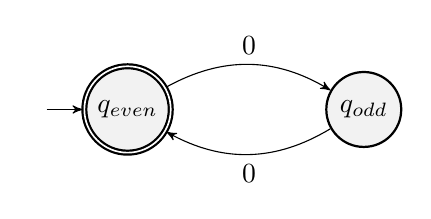
\begin{tikzpicture}
    \node[state, initial,accepting] (q1) {$q_{even}$};
    \node[state, right of=q1] (q2) {$q_{odd}$};
    \draw (q1) edge[bend left, above] node{0} (q2)
    (q2) edge[bend left, below] node{0} (q1);
  \end{tikzpicture}
\end{center}

A descrição formal do $AFD$ é:
\begin{center}
  $M_1 = (\{q_{even},q_{odd}\}, \{0\},\delta,q_{even}, \{q_{even}\})$
\end{center}
onde $\delta$ é representado da seguinte maneira:
\begin{table}[htbp]
  \centering
  \begin{tabular}{cclll}
    \multicolumn{1}{c|}{\textit{$\delta$}}   & \textit{0}                    & \textit{} & \textit{} & \textit{} \\ \cline{1-2}
    \multicolumn{1}{c|}{\textit{$q_{even}$}} & \textit{$q_{odd}$}            & \textit{} & \textit{} & \textit{} \\
    \multicolumn{1}{c|}{\textit{$q_{odd}$}}  & \textit{$q_{even}$}           & \textit{} & \textit{} & \textit{} \\
    \multicolumn{1}{l}{\textit{}}            & \multicolumn{1}{l}{\textit{}} & \textit{} & \textit{} & \textit{}
  \end{tabular}
\end{table}

\subsubsection*{(b) $L = \{(01)^n \ | \ n \in \mathbb{N}\}$}

\begin{center}
  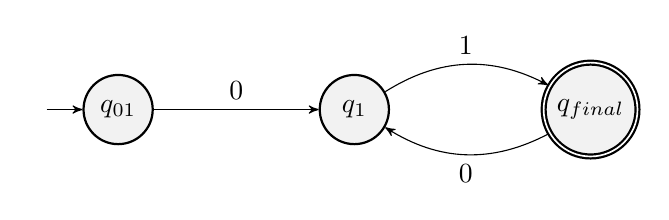
\begin{tikzpicture}
    \node[state, initial] (q1) {$q_{01}$};
    \node[state, right of=q1] (q2) {$q_{1}$};
    \node[state, accepting,right of=q2] (q3) {$q_{final}$};
    \draw (q1) edge[above] node{0} (q2)
    (q2) edge[bend left, above] node{1} (q3)
    (q3) edge[bend left, below] node{0} (q2);
  \end{tikzpicture}
\end{center}
\pagebreak
A descrição formal do $AFD$ é:
\begin{center}
  $M_2 = (\{q_{01},q_{1},q_{final}\}, \{0,1\},\delta,q_{01}, \{q_{final}\})$
\end{center}
onde $\delta$ é representado da seguinte maneira:
\begin{table}[htbp]
  \centering
  \begin{tabular}{c|ccll}
    \textit{$\delta$}    & \textit{0}       & \textit{1}           & \textit{} & \textit{} \\ \cline{1-3}
    \textit{$q_{01}$}    & \textit{$q_{1}$} & \textit{$\perp$}     & \textit{} & \textit{} \\
    \textit{$q_{1}$}     & \textit{$\perp$} & \textit{$q_{final}$} & \textit{} & \textit{} \\
    \textit{$q_{final}$} & \textit{$q_1$}   & \textit{$\perp$}     & \textit{} & \textit{}
  \end{tabular}
\end{table}

\subsubsection*{(c) A linguagem $L$ das strings sobre $\{0, 1\}$ que contêm pelos menos dois $0's$ e pelo menos um $1$.}

\begin{center}
  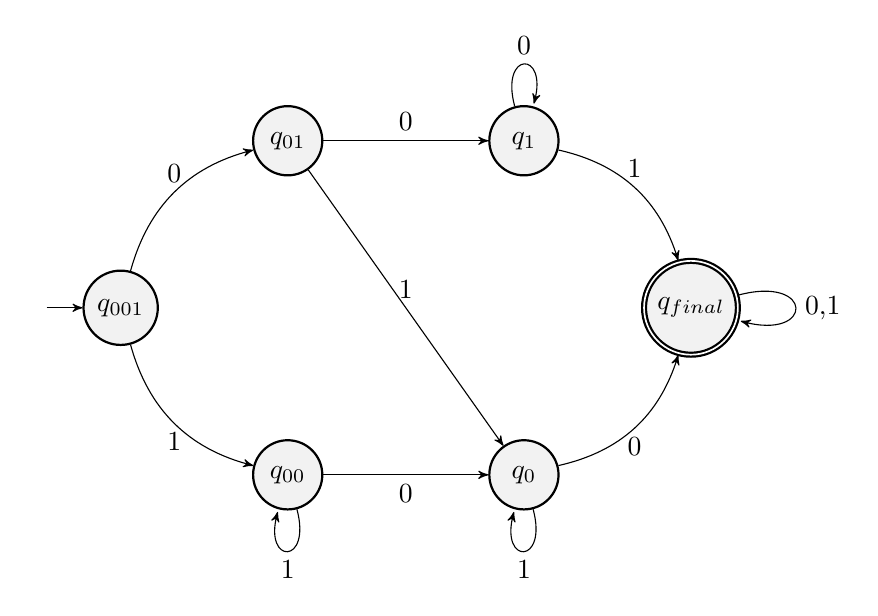
\begin{tikzpicture}
    \node[state, initial] (q001) {$q_{001}$};
    \node[state, above right of=q001] (q01) {$q_{01}$};
    \node[state, below right of=q001] (q00) {$q_{00}$};
    \node[state, right of=q01] (q1) {$q_{1}$};
    \node[state, right of=q00] (q0) {$q_{0}$};
    \node[state, accepting, below right of=q1] (qf) {$q_{final}$};
    \draw (q001) edge[bend left, above] node{0} (q01)
    (q001) edge[bend right, below] node{1} (q00)
    (q01) edge[above] node{0} (q1)
    (q01) edge[above] node{1} (q0)
    (q00) edge[below] node{0} (q0)
    (q00) edge[loop below] node{1} (q0)
    (q1) edge [bend left, above] node{1} (qf)
    (q1) edge [loop above] node{0} (q1)
    (q0) edge[bend right, below] node{0} (qf)
    (q0) edge[loop below] node{1} (q0)
    (qf) edge[loop right] node{0,1} (qf);
  \end{tikzpicture}
\end{center}

A descrição formal do $AFD$ é:
\begin{center}
  $M_3 = (\{q_{001},q_{01},q_{00},q_{1}, q_{0},q_{final}\}, \{0,1\},\delta,q_{001}, \{q_{final}\})$
\end{center}
onde $\delta$ é representado da seguinte maneira:
\begin{table}[htbp]
  \centering
  \begin{tabular}{c|cc}
    \textit{$\delta$}  & \textit{0}        & \textit{1}        \\ \hline
    \textit{$q_{001}$} & \textit{$q_{01}$} & \textit{$q_{00}$} \\
    \textit{$q_{00}$}  & \textit{$q_{0}$}  & \textit{$q_{00}$} \\
    \textit{$q_{01}$}  & \textit{$q_{1}$}  & \textit{$q_{0}$}  \\
    $q_{1}$            & $q_{1}$           & $q_{final}$       \\
    $q_{0}$            & $q_{final}$       & $q_{0}$           \\
    $q_{final}$        & $q_{final}$       & $q_{final}$
  \end{tabular}
\end{table}

\subsubsection*{(d) A linguagem $L$ das strings sobre $\{0, 1\}$ que contêm exatamente dois $0's$ e pelo menos dois $1's$.}

\begin{center}
  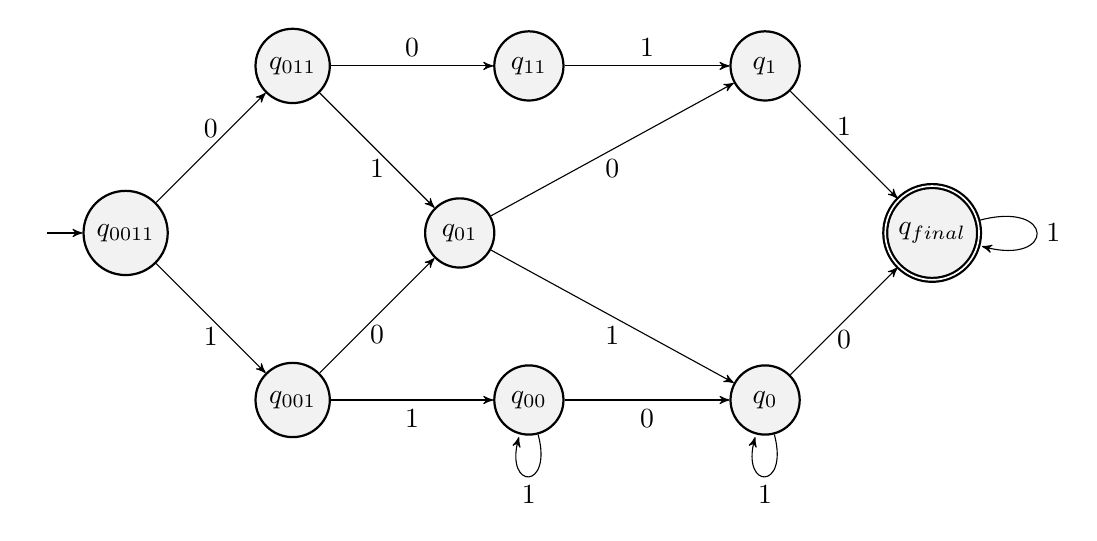
\begin{tikzpicture}
    \node[state, initial] (q0011) {$q_{0011}$};
    \node[state, above right of=q0011] (q011) {$q_{011}$};
    \node[state, below right of=q0011] (q001) {$q_{001}$};
    \node[state, right of=q011] (q11) {$q_{11}$};
    \node[state, below right of=q011] (q01) {$q_{01}$};
    \node[state, right of=q001] (q00) {$q_{00}$};
    \node[state, right of=q00] (q0) {$q_{0}$};
    \node[state, right of=q11] (q1) {$q_{1}$};
    \node[state, below right of=q1, accepting] (qf) {$q_{final}$};
    \draw (q0011) edge[above] node{0} (q011)
    (q0011) edge[below] node{1} (q001)
    (q011) edge[below] node{1} (q01)
    (q011) edge[above] node{0} (q11)
    (q001) edge[below] node{1} (q00)
    (q001) edge[below] node{0} (q01)
    (q01) edge[below] node{0} (q1)
    (q01) edge[below] node{1} (q0)
    (q11) edge[above] node{1} (q1)
    (q00) edge[below] node{0} (q0)
    (q00) edge[loop below] node{1} (q00)
    (q0) edge[loop below] node{1} (q0)
    (q0) edge[below] node{0} (qf)
    (q1) edge[above] node{1} (qf)
    (qf) edge[loop right] node{1} (qf);
  \end{tikzpicture}
\end{center}

A descrição formal do $AFD$ é:
\begin{center}
  $M_4 = (\{q_{0011},q_{011},q_{001},q_{11},q_{01},q_{00},q_{1}, q_{0},q_{final}\}, \{0,1\},\delta,q_{0011}, \{q_{final}\})$
\end{center}
onde $\delta$ é representado da seguinte maneira:

\begin{table}[htbp]
  \centering
  \begin{tabular}{c|cc}
    \textit{$\delta$}   & \textit{0}         & \textit{1}         \\ \hline
    \textit{$q_{0011}$} & \textit{$q_{011}$} & \textit{$q_{001}$} \\
    \textit{$q_{001}$}  & \textit{$q_{01}$}  & \textit{$q_{00}$}  \\
    \textit{$q_{011}$}  & \textit{$q_{11}$}  & \textit{$q_{01}$}  \\
    $q_{01}$            & $q_{0}$            & $q_{1}$            \\
    $q_{00}$            & $q_{0}$            & $q_{00}$           \\
    $q_{11}$            & $\perp$            & $q_{1}$            \\
    $q_{0}$             & $q_{final}$        & $q_{0}$            \\
    $q_{1}$             & $\perp$            & $q_{final}$        \\
    $q_{final}$         & $\perp$            & $q_{final}$
  \end{tabular}
\end{table}

\pagebreak

\subsubsection*{(e)  A linguagem $L$ das strings sobre $\{0, 1\}$ com um número par de $0's$ e um número ímpar de $1's$.}

\begin{center}
  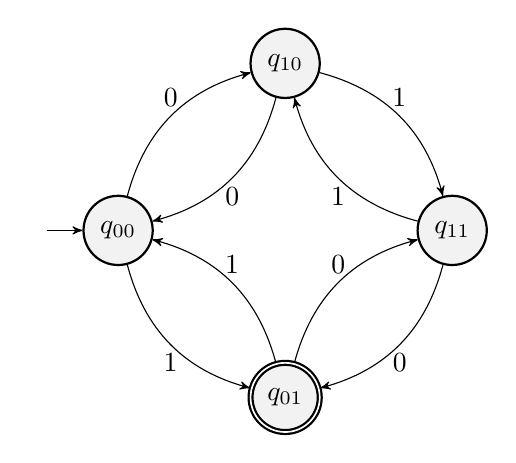
\begin{tikzpicture}
    \node[state, initial] (q00) {$q_{00}$};
    \node[state, above right of=q00] (q10) {$q_{10}$};
    \node[state, below right of=q00, accepting] (q01) {$q_{01}$};
    \node[state, above right of=q01] (q11) {$q_{11}$};
    \draw (q00) edge[bend left, above] node{0} (q10)
    (q00) edge[bend right, below] node{1} (q01)
    (q10) edge[bend left, below] node{0} (q00)
    (q10) edge[bend left, above] node{1} (q11)
    (q01) edge[bend right, above] node{1} (q00)
    (q01) edge[bend left, above] node{0} (q11)
    (q11) edge[bend left, below] node{0} (q01)
    (q11) edge[bend left, below] node{1} (q10);
  \end{tikzpicture}
\end{center}

A descrição formal do $AFD$ é:
\begin{center}
  $M_5 = (\{q_{00},q_{10},q_{01},q_{11}\}, \{0,1\},\delta,q_{00}, \{q_{01}\})$
\end{center}
onde $\delta$ é representado da seguinte maneira:
\begin{table}[htbp]
  \centering
  \begin{tabular}{c|cc}
    \textit{$\delta$} & \textit{0}        & \textit{1}        \\ \hline
    \textit{$q_{00}$} & \textit{$q_{10}$} & \textit{$q_{01}$} \\
    \textit{$q_{10}$} & \textit{$q_{00}$} & \textit{$q_{11}$} \\
    \textit{$q_{01}$} & \textit{$q_{11}$} & \textit{$q_{00}$} \\
    $q_{11}$          & $q_{01}$          & $q_{10}$
  \end{tabular}
\end{table}

\subsubsection*{(f) A linguagem $L$ das strings sobre $\{0, 1\}$ que não contêm a substring $010$.}

\begin{center}
  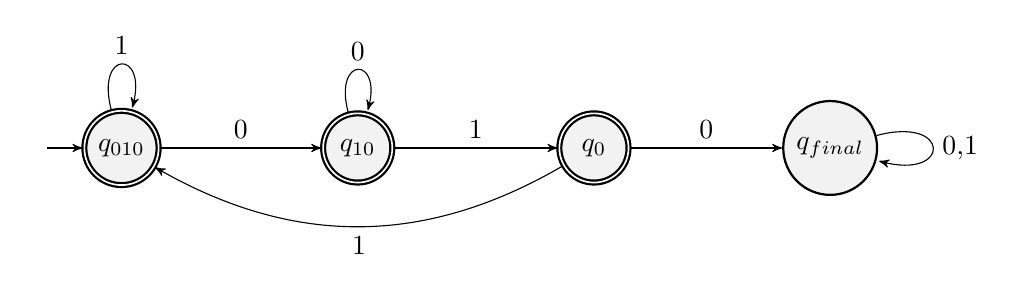
\begin{tikzpicture}
    \node[state, initial, accepting] (q010) {$q_{010}$};
    \node[state, accepting, right of=q010] (q10) {$q_{10}$};
    \node[state, accepting, right of=q10] (q0) {$q_{0}$};
    \node[state, right of=q0] (qf) {$q_{final}$};
    \draw (q010) edge[loop above] node{1} (q010)
    (q010) edge[above] node{0} (q10)
    (q10) edge[loop above] node{0} (q10)
    (q10) edge[above] node{1} (q0)
    (q0) edge[above] node{0} (qf)
    (q0) edge[bend left, below] node{1} (q010)
    (qf) edge[loop right] node{0,1} (qf);
  \end{tikzpicture}
\end{center}

A descrição formal do $AFD$ é:
\begin{center}
  $M_6 = (\{q_{010},q_{10},q_{0},q_{final}\}, \{0,1\},\delta,q_{010}, \{q_{010},q_{10},q_{0}\})$
\end{center}
\pagebreak
onde $\delta$ é representado da seguinte maneira:

\begin{table}[htbp]
  \centering
  \begin{tabular}{c|cc}
    \textit{$\delta$}  & \textit{0}           & \textit{1}         \\ \hline
    \textit{$q_{010}$} & \textit{$q_{10}$}    & \textit{$q_{010}$} \\
    \textit{$q_{10}$}  & \textit{$q_{10}$}    & \textit{$q_{0}$}   \\
    \textit{$q_{0}$}   & \textit{$q_{final}$} & \textit{$q_{010}$} \\
    $q_{final}$        & $q_{final}$          & $q_{final}$
  \end{tabular}
\end{table}

\subsubsection*{(g) A linguagem $L$ das strings sobre $\{0, 1\}$ com um número par de $0's$ e em que cada $0$ é sempre seguido de pelo menos um $1$.}

\begin{center}
  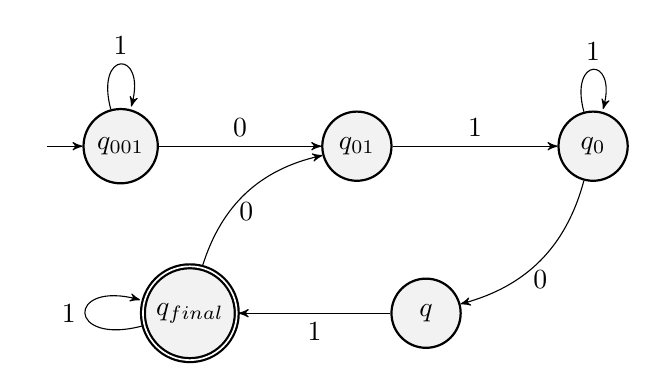
\begin{tikzpicture}
    \node[state, initial] (q001) {$q_{001}$};
    \node[state, right of=q001] (q01) {$q_{01}$};
    \node[state, right of=q01] (q0) {$q_{0}$};
    \node[state, below left of=q0] (q) {$q$};
    \node[state, accepting,left of=q] (qf) {$q_{final}$};
    \draw (q001) edge[loop above] node{1} (q001)
    (q001) edge[above] node{0} (q01)
    (q01) edge[above] node{1} (q0)
    (q0) edge[loop above] node{1} (q0)
    (q0) edge[bend left, below] node{0} (q)
    (q) edge[below] node{1} (qf)
    (qf) edge[bend left, below] node{0} (q01)
    (qf) edge[loop left] node{1} (qf);
  \end{tikzpicture}
\end{center}

A descrição formal do $AFD$ é:
\begin{center}
  $M_7 = (\{q_{001},q_{01},q_{0},q,q_{final}\}, \{0,1\},\delta,q_{001}, \{q_{final}\})$
\end{center}
onde $\delta$ é representado da seguinte maneira:

\begin{table}[htbp]
  \centering
  \begin{tabular}{c|cc}
    \textit{$\delta$}  & \textit{0}        & \textit{1}         \\ \hline
    \textit{$q_{001}$} & \textit{$q_{01}$} & \textit{$q_{001}$} \\
    \textit{$q_{01}$}  & \textit{$\perp$}  & \textit{$q_{0}$}   \\
    \textit{$q_{0}$}   & \textit{$q$}      & \textit{$q_{0}$}   \\
    $q$                & $\perp$           & $q_{final}$        \\
    $q_{final}$        & $q_{01}$          & $q_{final}$
  \end{tabular}
\end{table}

\pagebreak

\subsubsection*{(h) A linguagem L das strings sobre $\{0\}$ com tamanho divisível por $2$ ou por $3$.}

$q_{ij}$ onde $i = n \% 2$ e $j = n \% 3$.

\begin{center}
  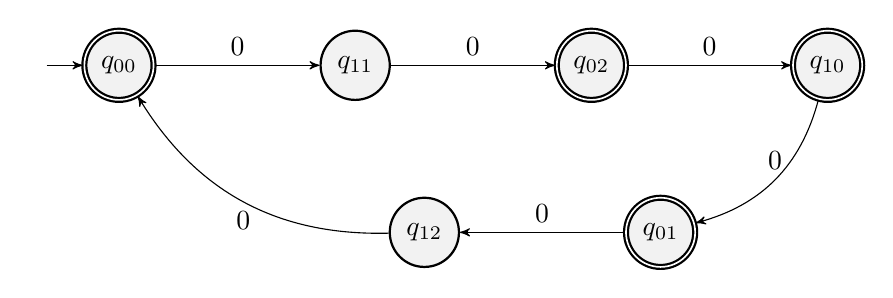
\begin{tikzpicture}
    \node[state, accepting, initial] (q00) {$q_{00}$};
    \node[state, right of=q00] (q11) {$q_{11}$};
    \node[state, accepting, right of=q11] (q02) {$q_{02}$};
    \node[state, accepting, right of=q02] (q10) {$q_{10}$};
    \node[state, accepting, below left of=q10] (q01) {$q_{01}$};
    \node[state, left of=q01] (q12) {$q_{12}$};
    \draw (q00) edge[above] node{0} (q11)
    (q11) edge[above] node{0} (q02)
    (q02) edge[above] node{0} (q10)
    (q10) edge[bend left, above] node{0} (q01)
    (q01) edge[above] node{0} (q12)
    (q12) edge[bend left, below] node{0} (q00);
  \end{tikzpicture}
\end{center}

A descrição formal do $AFD$ é:
\begin{center}
  $M_8 = (\{q_{00},q_{11},q_{02},q_{10},q_{01},q_{12}\}, \{0\},\delta,q_{00}, \{q_{00},q_{02},q_{10},q_{01}\})$
\end{center}
onde $\delta$ é representado da seguinte maneira:
\begin{table}[htbp]
  \centering
  \begin{tabular}{c|c}
    \textit{$\delta$} & \textit{0}        \\ \hline
    \textit{$q_{00}$} & \textit{$q_{11}$} \\
    \textit{$q_{11}$} & \textit{$q_{02}$} \\
    \textit{$q_{02}$} & \textit{$q_{10}$} \\
    $q_{10}$          & $q_{01}$          \\
    $q_{01}$          & $q_{12}$          \\
    $q_{12}$          & $q_{00}$
  \end{tabular}
\end{table}

\subsubsection*{(i) A linguagem $L$ das strings sobre $\{A, C, G, T \}$ que contêm pelo menos uma ocorrência da substring $ACT$.}

\begin{center}
  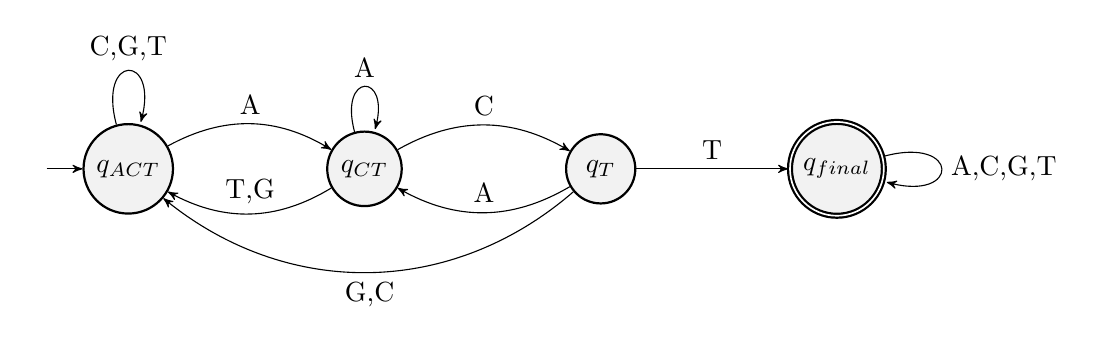
\begin{tikzpicture}
    \node[state, initial] (q0) {$q_{ACT}$};
    \node[state, right of=q0] (q1) {$q_{CT}$};
    \node[state, right of=q1] (q2) {$q_{T}$};
    \node[state, right of=q2, accepting] (qf) {$q_{final}$};
    \draw (q0) edge[loop above] node{C,G,T} (q0)
    (q0) edge[bend left, above] node{A} (q1)
    (q1) edge[loop above] node{A} (q1)
    (q1) edge[bend left, above] node{T,G} (q0)
    (q1) edge[bend left, above] node{C} (q2)
    (q2) edge[bend left, above] node{A} (q1)
    (q2) edge[above] node{T} (qf)
    (qf) edge[loop right] node{A,C,G,T} (qf)
    (q2) edge[bend left=40, below] node{G,C} (q0);
  \end{tikzpicture}
\end{center}

\pagebreak

A descrição formal do $AFD$ é:
\begin{center}
  $M_9 = (\{q_{ACT},q_{CT},q_{T},q_{final}\}, \{A,C,G,T\},\delta,q_{ACT}, \{q_{final}\})$
\end{center}
onde $\delta$ é representado da seguinte maneira:

\begin{table}[htbp]
  \centering
  \begin{tabular}{c|cccc}
    \textit{$\delta$} & \textit{A}  & C           & G           & T           \\ \hline
    $q_{ACT}$         & $q_{CT}$    & $q_{ACT}$   & $q_{ACT}$   & $q_{ACT}$   \\
    $q_{CT}$          & $q_{CT}$    & $q_{T}$     & $q_{ACT}$   & $q_{ACT}$   \\
    $q_{T}$           & $q_{CT}$    & $q_{ACT}$   & $q_{ACT}$   & $q_{final}$ \\
    $q_{final}$       & $q_{final}$ & $q_{final}$ & $q_{final}$ & $q_{final}$
  \end{tabular}
\end{table}

\subsubsection*{(j) $L = \varnothing $}
Iremos assumir $\Sigma$ como $\{0,1\}$.

\begin{center}
  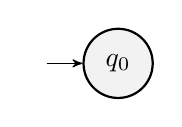
\begin{tikzpicture}
    \node[state, initial] (q0) {$q_0$};
  \end{tikzpicture}
\end{center}

A descrição formal do $AFD$ é:
\begin{center}
  $M_{10} = (\{q_{0}\}, \{0,1\},\delta,q_{0}, \varnothing)$
\end{center}
onde $\delta$ é representado da seguinte maneira: $\delta:S\times \Sigma\to S$ dada por $\delta(q_0,0)=\bot$ e $\delta(q_0,1)=\bot$

\subsubsection*{(k) $L = {\varepsilon}$ }

Iremos assumir $\Sigma$ como $\{0,1\}$.

\begin{center}
  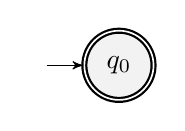
\begin{tikzpicture}
    \node[state, initial, accepting] (q0) {$q_0$};
  \end{tikzpicture}
\end{center}

A descrição formal do $AFD$ é:
\begin{center}
  $M_{11} = (\{q_{0}\}, \{0,1\},\delta, q_{0}, \{q_0\})$
\end{center}
onde $\delta$ é representado da seguinte maneira: $\delta:S\times \Sigma\to S$ dada por $\delta(q_0,0)=\bot$ e $\delta(q_0,1)=\bot$

\subsubsection*{(l) $L = \{0, 1\}^{*} \setminus \{\varepsilon\}$}

\begin{center}
  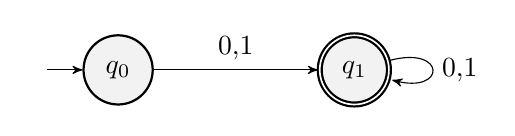
\begin{tikzpicture}
    \node[state, initial] (q0) {$q_{0}$};
    \node[state, right of=q0, accepting] (q1) {$q_{1}$};
    \draw (q0) edge[above] node{0,1} (q1)
    (q1) edge[loop right] node{0,1} (q1);
  \end{tikzpicture}
\end{center}

A descrição formal do $AFD$ é:
\begin{center}
  $M_{12} = (\{q_{0},q_1\}, \{0,1\},\delta, q_{0}, \{q_1\})$
\end{center}

\pagebreak

onde $\delta$ é representado da seguinte maneira:
\begin{table}[htbp]
  \centering
  \begin{tabular}{c|cc}
    \textit{$\delta$} & \textit{0} & 1       \\ \hline
    $q_{0}$           & $q_{1}$    & $q_{1}$ \\
    $q_{1}$           & $q_{1}$    & $q_{1}$
  \end{tabular}
\end{table}

\subsection*{Exercício 2}
Para cada um dos $AFD's$ que construiu nas alíneas (a) a (g) do Exercício 1, descreva a sequência de estados percorridos no input $0100110$ e diga se esta string é aceite ou não.

\subsubsection*{(a)}
$\delta(q_{even}, 0100110) = \delta(\delta(q_{even}, 0), 1001110) = \delta(\delta(q_{odd}, 1), 001110)$, $\delta(q_{odd}, 1) = \bot$. logo esta sequência não é aceite.

\subsubsection*{(b)}
$\delta(q_{01}, 0100110) = \delta(\delta(q_{01}, 0), 100110) = \delta(\delta(q_{1}, 1), 00110) = \delta(\delta(q_{final}, 0), 0110) = delta(\delta(q_{1}, 0), 110)$ como $ \delta(q_{1}, 0) = \bot$, a sequência não é aceite.

\subsubsection*{(c)}
$\delta(q_{001}, 0100110) = \delta(\delta(q_{001}, 0), 100110) = \delta(\delta(q_{01}, 1), 00110) = \delta(\delta(q_{0}, 0), 0110) = \delta(\delta(q_{final}, 0), 110) = \delta(\delta(q_{final}, 1), 10) = \delta(\delta(q_{final}, 1), 0) =
  \delta(q_{final}, 0) = q_{final}$, como $q_{final} \in F$, a sequência é aceite.

\subsubsection*{(d)}
$\delta(q_{0011}, 0100110) = \delta(\delta(q_{0011}, 0), 100110) = \delta(\delta(q_{011}, 1), 00110) = \delta(\delta(q_{01}, 0), 0110) = \delta(\delta(q_{1}, 0), 110)$, como $\delta(q_{1}, 0) = \bot$, a sequência não é aceite.

\subsubsection*{(e)}
$\delta(q_{00}, 0100110) = \delta(\delta(q_{00}, 0), 100110) = \delta(\delta(q_{10}, 1), 00110) = \delta(\delta(q_{11}, 0), 0110) = \delta(\delta(q_{01}, 0), 110) = \delta(\delta(q_{11}, 1), 10) = \delta(\delta(q_{10}, 1), 0) = \delta(q_{11}, 0) = q_{01}$, como $q_{01} \in F$, a sequência é aceite.

\subsubsection*{(f)}
$\delta(q_{010}, 0100110) = \delta(\delta(q_{010}, 0), 100110) = \delta(\delta(q_{10}, 1), 00110) = \delta(\delta(q_{0}, 0), 0110) = \delta(\delta(q_{final}, 0), 110) = \delta(\delta(q_{final}, 1), 10) = \delta(\delta(q_{final}, 1), 0) = \delta(q_{final}, 1) = q_{final}$, como $q_{final} \notin F$, a sequência não é aceite.

\subsubsection*{(g)}
$\delta(q_{001}, 0100110) = \delta(\delta(q_{001}, 0), 100110) = \delta(\delta(q_{01}, 1), 00110) = \delta(\delta(q_{0}, 0), 0110) = \delta(\delta(q, 0), 110)$, como $\delta(q, 0) = \bot$, a sequência não é aceite.


\subsection*{Exercício 3}
\subsubsection*{Seja $L$ uma linguagem regular. Quando é que temos $\epsilon \in L$?}

Se $L$ é regular quer dizer que existe um $AFD$ $M = (S,\Sigma,\delta,s,F)$ com função de transição total que reconhece $L$. Para $M$ reconhecer $\epsilon$, basta termos $s \in F$. Ou seja o estado inicial também ser estado de aceitação.

\subsection*{Exercício 4}
Para cada uma das linguagens $L$ abaixo descreva um $AFD$ que a reconhece através do seu diagrama de estados. Sugestão: Primeiro construa um $AFD$ que reconhece o complemento $\overline{L}$ e depois converta-o para um $AFD$ que reconhece $L$.
\subsubsection*{(a) A linguagem $L$ sobre $\{a, b\}$ cujas strings não contêm a substring $ab$.}

\begin{center}
  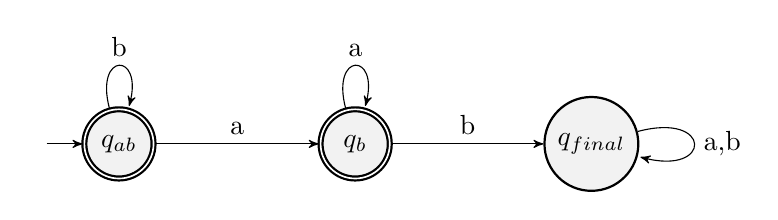
\begin{tikzpicture}
    \node[state, initial, accepting] (qab) {$q_{ab}$};
    \node[state, accepting, right of=qab] (qb) {$q_b$};
    \node[state, right of=qb] (qf) {$q_{final}$};
    \draw (qab) edge[above] node{a} (qb)
    (qab) edge[loop above] node{b} (qab)
    (qb) edge[above] node{b} (qf)
    (qb) edge[loop above] node{a} (qb)
    (qf) edge[loop right] node{a,b} (qf);
  \end{tikzpicture}
\end{center}

\subsubsection*{(b) $L = \{a, b\}^\ast \setminus \{a^{m}b^n \ | \ m, n \in \mathbb{N}\}$}

\begin{center}
  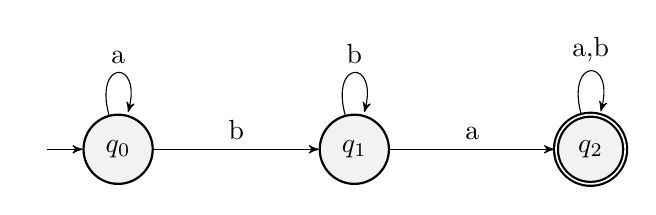
\begin{tikzpicture}
    \node[state, initial] (q0) {$q_{0}$};
    \node[state, right of=q0] (q1) {$q_{1}$};
    \node[state, right of=q1, accepting] (q2) {$q_{2}$};
    \draw (q0) edge[above] node{b} (q1)
    (q0) edge[loop above] node{a} (q0)
    (q1) edge[above] node{a} (q2)
    (q1) edge[loop above] node{b} (q1)
    (q2) edge[loop above] node{a,b} (q2);
  \end{tikzpicture}
\end{center}

\subsubsection*{(c) $L = \{a, b\}^\ast \setminus (\{a\}^\ast \cup \{b\}^
    \ast)$}

\begin{center}
  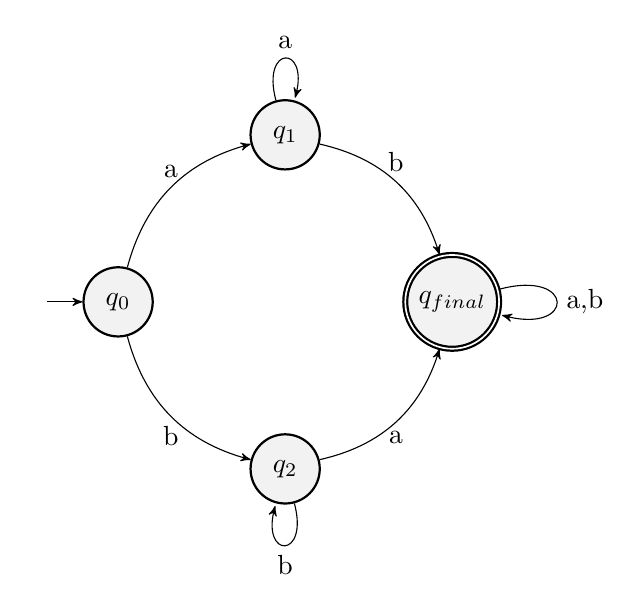
\begin{tikzpicture}
    \node[state, initial] (q0) {$q_{0}$};
    \node[state, above right of=q0] (q1) {$q_{1}$};
    \node[state, below right of=q0] (q2) {$q_{2}$};
    \node[state, accepting ,below right of=q1] (qf) {$q_{final}$};
    \draw (q0) edge[bend left, above] node{a} (q1)
    (q0) edge[bend right, below] node{b} (q2)
    (q1) edge[loop above] node{a} (q1)
    (q2) edge[loop below] node{b} (q2)
    (q1) edge[bend left,above] node{b} (qf)
    (q2) edge[bend right, below] node{a} (qf)
    (qf) edge[loop right] node{a,b} (qf);
  \end{tikzpicture}
\end{center}

\subsubsection*{(d)  A linguagem $L$ sobre $\{a, b\}$ cujas strings não contêm exatamente dois $a's$.}

\begin{center}
  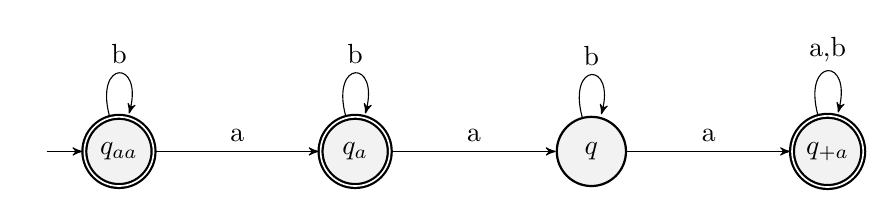
\begin{tikzpicture}
    \node[state, initial, accepting] (qaa) {$q_{aa}$};
    \node[state, accepting, right of=qaa] (qa) {$q_{a}$};
    \node[state, right of=qa] (q) {$q$};
    \node[state, accepting, right of=q] (q+a) {$q_{+a}$};
    \draw (qaa) edge[loop above] node{b} (qaa)
    (qaa) edge[above] node{a} (qa)
    (qa) edge[loop above] node{b} (qa)
    (qa) edge[above] node{a} (q)
    (q) edge[loop above] node{b} (q)
    (q) edge[above] node{a} (q+a)
    (q+a) edge[loop above] node{a,b} (q+a);
  \end{tikzpicture}
\end{center}

\subsection*{Exercício 5}
\subsubsection*{Sejam $L_1$ e $L_2$ linguagens regulares sobre o mesmo alfabeto $\Sigma$. Mostre que $L_1 \cap L_2$ também é regular.}

Como $L_1$ e $L_2$ são regulares, existem $AFD's \ M_1 = (S_1, \Sigma, \delta_1, s_1, F_1)$ e $M_2 = (S_2, \Sigma, \delta_2, s_2, F_2)$, com funções de transição $\delta_1 $ e $ \delta_2$ totais tal que $M_1$ e $M_2$ aceitam $L_1$ e $L_2$ respetivamente. Queremos construir um $AFD \ M$ a partir de $M_1$ e $M_2$ que reconhece $L_1 \cap L_2$. Dado um input $w$, queremos simular as computações de $M_1$ e $M_2$ em $w$ lado-a-lado, e aceitar $w$ exatamente quando ambos $M_1$ e $M_2$ aceitam $w$.

Para implementar a estratégia acima vamos definir um novo $AFD \ M = (S, \Sigma, \delta, s, F)$. Para tal necessitamos de a cada momento saber os estados atuais de $M_1$ e $M_2$ na computação. Ou seja os estados de $M$ podem ser descritos como \textit{pares} de estados de $M_1$ e $M_2$, em que cada par representam o estado atual dos dois $AFD's$. Portanto queremos $S = S_1 \times S_2$. Se $M$ estiver no estado $(q_1,q_2) \in S_1 \times S_2$ num dado ponto da computação e ler o símbolo $a \in \Sigma$, queremos simular a computação de $M_1$ e $M_2$, para tal deveríamos atualizar $q_1$ para $\delta_1(q_1, a)$ e $q_2$ para $\delta_2(q_2, a)$. Definimos então a função de transição $\delta$ como
\[
  \delta((q_1,q_2),a) = (\delta_1(q_1, a), \delta_2(q_2, a)).
\]
Para o estado inicial de $M$, queremos escolher o par de estados iniciais de $M_1$ e $M_2$. Escrevemos então $s = (s_1,s_2)$. Resta especificar $F$, o conjunto de estados finais de $M$. Queremos aceitar $w$ se ambas as computação de $M_1$ e $M_2$ acabarem em estados de aceitação. Para tal queremos escolher $F$ como o conjunto de pares $(q_1,q_2) \in S$ tal que $q_1 \in F_1 $ e $q_2 \in F_2$. Ou seja definimos o conjunto de estados de aceitação $F$ como
\[
  F = (F_1 \times F_2)
\]
Agora que definimos $M$ formalmente, queremos provar que $L(M) = L_1 \cap L_2$.Para tal vamos mostrar $L(M) \subseteq L_1 \cap L_2$ e $L_1 \cap L_2 \subseteq L(M)$. Comecemos por supor que $w \in \Sigma^\ast$, arbitrário. Denotemos a sequência de estados gerada por $w$ em $M_i$ por $(r_0^{(i)},r_1^{(i)},\dots,r_n^{(i)})$ para $i \in \{1,2\}$ e $n \in \mathbb{N}$. Se $w \in L_1 \cap L_2$, pela definição de $M_1$ e $M_2$ temos que $r_n^{(1)} \in F_1 $ e $r_n^{(2)} \in F_2$. Deste modo concluímos que $\delta(w) = (r_n^{(1)}, r_n^{(2)}) \in F$. Como $W$ é arbitrário, segue que $L_1 \cap L_2 \subseteq L(M)$. Por outro lado, se $w \notin L_1 \cap L_2$, então temos que $r_n^{(1)} \notin F_1 $ e $r_n^{(2)} \notin F_2$, o que leva a $(r_n^{(1)}, r_n^{(2)}) \notin F$, portanto $w \notin L(M)$. Logo, $L(M) \subseteq L_1 \cap L_2$, e concluímos que $L(M) = L_1 \cap L_2$.

\subsection*{Exercício 6}
\subsubsection*{Dada uma string $w = w_1w_2\dots w_n \in \Sigma^\ast$ definimos o seu reverso $rev(w) = w_{n}w_{n-1}\dots w_2w_1$. Para uma linguagem $L \subseteq \Sigma^\ast$, definimos $rev(L) = {rev(w) | w \in L}$. Mostre que se $L$ é regular então $rev(L)$ também é regular.}

Resolver com um AFN .-.

\subsection*{Exercício 7}
\subsubsection*{Seja $L_n = \{0^k | \ k $ é múltiplo de $n \}$. Mostre que $L_n$ é regular para qualquer $n \in \mathbb{N}^+$.}

Fixamos $n \in \mathbb{N}^+$. Queremos mostrar que o $AFD \ M = (S,\Sigma,\delta,s,F)$, reconhece $L_n$ \textit{i.e} $L(M) = L_n$.

\begin{center}
  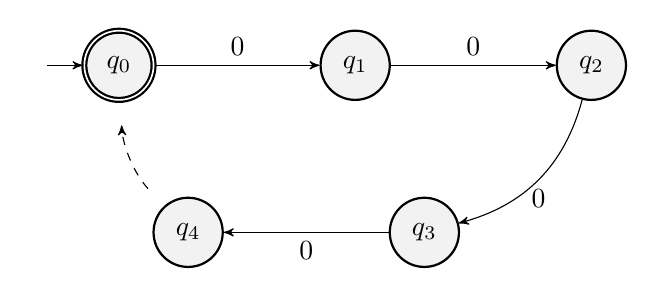
\begin{tikzpicture}
    \node[state, initial, accepting] (q0) {$q_0$};
    \node[state, right of= q0] (q1) {$q_1$};
    \node[state, right of= q1] (q2) {$q_2$};
    \node[state, below left of= q2] (q3) {$q_3$};
    \node[state, left of= q3] (q4) {$q_4$};
    \draw[dashed, shorten <=3mm, shorten >=3mm] (q4) to[bend left=20] (q0);
    \draw (q0) edge[above] node{0} (q1)
    (q1) edge[above] node{0} (q2)
    (q2) edge[bend left, below] node{0} (q3)
    (q3) edge[below] node{0} (q4);
  \end{tikzpicture}
\end{center}

Vamos definir $M$. Comecemos pelo conjunto de estados $S$. Queremos cobrir todos os multiplos possíveis, comecando no $q_0$, para tal vamos ter $m - 1$ estados tal que $m$ é o número de multiplos possíveis ou seja, $S = \{q_0,q_1,q_2,\dots , q_{m-1}\}$. Intuitivamente $\Sigma = 0$. O estado inicial $q$ será o estado $q_0$, portanto $s=q_0$. O conjunto de estados finais $F$ é dado por um único estado $q_0$ o que se traduz para $F = \{q_0\}$. Falta nos então definir $\delta$. Em cada estado $q_i \in S$ queremos ler o símbolo $'0'$ repetindo ciclicamente até chegar ao estado final $q_0$. Portanto obtemos:
\[
  \delta(q_i,0) = q_{(i+1) \% n}
\]
Desta forma, $M$ reconhece sequência de potências de $0$ cujo expoente seja um múltiplo de $n$. Portanto agora falta-nos provar que $L(M) = L_n$. Para tal vamos demonstrar que $L(M) \subseteq L_n$ e $L_n \subseteq L(M)$. Comecemos por supor que $w \in \Sigma^\ast$, arbitrário. Denotemos a sequência de estados gerado por $w$ em $M$ por $(q_0,q_1,q_2,\dots , q_{i})$ com $i \in \mathbb{N}$. Se $w \in L_n$ pela definição de $L_n \ , q_i \in F$. Como $F = \{q_0\}$, $q_i = q_0$. Ou seja $\delta(w) = q_0 \in F$. Visto que $w$ é arbitrário, segue que $L_n \subseteq L(M)$. Por outro lado, se $w \notin L_n$ então $q_i \notin F$, pelo que $q_i \neq q_0$. Como $F = \{q_0\}$ e $q_i \neq q_0$, $w \notin L(M)$. Logo, $L(M) \subseteq L_n$, e concluímos que $L(M) = L_n$.

\end{document}